\documentclass[prd,preprint]{revtex4}

\usepackage{amsmath}
\usepackage{hyperref}
\usepackage{color}
\usepackage{graphicx}

\newcommand{\vtheta}{\vec{\theta}}

\newcommand{\be}{\begin{equation}}
\newcommand{\ee}{\end{equation}}
\newcommand{\bel}[1]{\begin{equation}\label{#1}}
\newcommand{\ba}{\begin{eqnarray}}
\newcommand{\ea}{\end{eqnarray}}
\newcommand{\bal}[1]{\begin{eqnarray}\label{#1}}

\newcommand{\ilya}[1]{{\color{red} \bf Ilya: #1}}
\newcommand{\will}[1]{{\color{blue} \bf Will: #1}}


\bibliographystyle{h-physrev}

\begin{document}
\title{An Efficient Interpolation Technique for Jump Proposals in
  Reversible-Jump Markov Chain Monte Carlo Calculations}

\date{\today}

\author{Will M. Farr}
\email{w-farr@northwestern.edu}

\affiliation{Northwestern University Center for Interdisciplinary
  Research and Education in Astrophysics}

\author{Ilya Mandel}
\email{ilyamandel@chgk.info}

\affiliation{MIT Kavli Institute; and University of Birmingham, UK}

\begin{abstract}
  \ilya{Add physics/astro motivation} Reversible-jump Markov chain
  monte carlo (RJMCMC) is an extremely powerful technique for
  performing Bayesian model selection, but it suffers from a
  fundamental difficulty: it requires jumps between model parameter
  spaces, but cannot retain a memory of the favored locations in more
  than one parameter space at a time.  Thus, a naive jump between
  parameter spaces is unlikely to be accepted in the MCMC algorithm
  and convergence is correspondingly slow.  Here we demonstrate an
  interpolation technique that uses samples from single-model MCMCs to
  propose inter-model jumps from an approximation to the single-model
  posterior of the target parameter space.  The interpolation
  technique, based on a kD-tree data structure, is adaptive and
  efficient in arbitrary dimensions.  We show that our technique leads
  to dramatically improved convergence over naive jumps in an RJMCMC,
  and compare it to other proposals in the literature to improve the
  convergence of RJMCMCs.  We also discuss the use of the same
  interpolation technique in two other contexts: as a convergence test
  for a single-model MCMC and as a way to construct efficient
  ``global'' proposal distributions for single-model MCMCs without
  prior knowledge of the structure of the posterior distribution.
\end{abstract}

\maketitle

\section{Introduction}

\will{Mention Weinberg direct integration (Ref.~\cite{Weinberg2009}).}

\section{Reversible Jump MCMC}

Reversible jump Markov chain Monte Carlo (RJMCMC) \cite{Green1995} is a technique for Bayesian model comparison.  Below, we give a very brief introduction to Bayesian analysis; describe a standard MCMC; and introduce RJMCMC.

\subsection{Bayesian analysis}

Consider an observed data set $d$ and a set of competing models for
the data, indexed by an integer $i$: $\{M_i | i = 1, 2, \ldots \}$.
Each model has some continuous parameters, $\vtheta_i$; given the
model and its parameters, we can make a prediction about the
likelihood of observing the experimental data: $L(d|\vtheta_i, M_i)$.
Within the framework of each model, Bayes' rule gives us a way to
compute the posterior probability distribution function (PDF) for the
model parameters implied by the data:
\be
  p(\vtheta_i | d, M_i) = \frac{L(d|\vtheta_i, M_i) p(\vtheta_i|M_i)}{p(d|M_i)},
\ee
where $p(\vtheta_i |d, M_i)$ is the posterior distribution for the
model parameters $\vtheta_i$ implied by the data in the context of
model $M_i$, $p(\vtheta_i|M_i)$ is the prior probability of the model
parameters that represents our beliefs before accumulating any of the
data $d$, and $p(d|M_i)$, called the evidence, is an overall
normalizing constant that ensures that $p(\vtheta_i|d,M_i)$ is
properly normalized as a probability distribution on the $\vtheta_i$.
This implies that the evidence is equal to
\bel{evidence}
  p(d|M_i) = \int_{V_i} d\vtheta_i L(d|\vtheta_i, M_i) p(\vtheta_i|M_i),
\ee
where $V_i$ is the parameter space volume in model $M_i$.  For model
comparison, we are interested in the posterior probability of a
particular model, $M_i$, given the data, $p(M_i|d)$.  Using Bayes'
rule, we see that this involves the evidence (Eq.~\eqref{evidence}):
\be
p(M_i|d) = \frac{p(d|M_i) p(M_i)}{p(d)},
\ee
where $p(M_i)$ is our a priori belief in model $M_i$ and $p(d)$ is a
normalizing constant,
\be
p(d)=\sum_i p(d|M_i) p(M_i).
\ee

When selecting among alternative models, we are interested in finding
the model with the highest posterior probability $p(M_i|d)$.  However,
attempts to directly compute the evidence by performing the
integration in Eq.~\eqref{evidence} are generally very difficult in a
multi-dimensional, multi-modal parameter space when the likelihood has
to be evaluated numerically.  In particular, a grid-based integral
quickly becomes computationally unfeasible as the dimensionality of
$\vtheta$ exceeds a few.  The parameter space must typically be
explored in a stochastic manner before the evidence integral can be
computed.  There are several stochastic parameter-exploration
techniques focused directly on evidence computation (e.g., nested
sampling and MultiNest \ilya {Add references}).  However, we
frequently want to compute the posterior PDFs within each model along
with the evidences for the various models.  One of the most common
techniques for computing posterior PDFs in the context of a model is
the Markov Chain Monte Carlo, which we now describe.

\subsection{MCMC} \label{sec:mcmc}

\will{Here $i$ should become $j$ (or some other index), because we
  have used $i$ already to denote the model.}

A Markov chain Monte Carlo produces a set of samples $\{ \vtheta^{(i)} \, | \, i = 1, \ldots \}$ from the model parameter space that are sampled according to the posterior, meaning that, in the limit that the chain length tends to infinity, the relative frequency with which a given set of parameter appears in the chain is proportional to the desired posterior, $p(\vtheta|d,M)$.  Therefore, the output of an MCMC can be directly interpreted as the posterior PDF over the full parameter space, while PDFs for individual parameters can be obtained through trivially marginalizing over the uninteresting parameters, simply by considering the distribution of the parameter of interest in the MCMC samples.

A Markov chain has the property that the probability distribution of the next state can depend only on the current state, not on the past history:
\be
p(\vtheta^{(i+1)})=\int_{V} d\vtheta^{i} p(\vtheta^{(i)} \to \vtheta^{(i+1)}) p(\vtheta^{(i+1)}),
\ee
where $p(\vtheta^{(i)} \to \vtheta^{(i+1)})$ depends only on $\vtheta^{(i)}$ and $\vtheta^{(i+1)}$. 
An additional requirement for an MCMC arises from the fact that the desired distribution is the equilibrium distribution.  In other words, if we assume that state $(i)$ of the chain is sampled from the desired PDF, $p(\vtheta^{(i)})=p(\vtheta|d,M)$ , then the next state $(i+1)$ must be sampled from the PDF as well, so that $p(\vtheta^{(i+1)})=p(\vtheta|d,M)$.  

One way to produce such a sequence of samples is via the Metropolis-Hastings algorithm, first proposed by Metropolis et al.~in 1953 \cite{Metropolis:1953}, and later generalized by Hastings:
\begin{enumerate}
  \item Given a current state $\vtheta^{(i)}$, propose the next state $\vtheta^p$ by drawing from a jump proposal distribution with probability $Q(\vtheta^{(i)} \to \vtheta^p)$.  
  \item Compute the probability of accepting the proposed jump as
\be
p_{\textnormal{accept}}  \equiv \min\Bigl(1,  \frac{p(\vtheta^p|d)}{p(\vtheta^{(i)}|d)} \frac{Q(\vtheta^p \to
        \vtheta^{(i)})}{Q(\vtheta^{(i)} \to \vtheta^p)} \Bigr).
\ee
\item Pick a uniform random number $\alpha \in [0,1]$.  If $\alpha<  p_{\textnormal{accept}}$, accept the proposed jump, setting $\vtheta^{(i+1)}=\vtheta^p$.  Otherwise, reject the jump, and remain at the same location in parameter space for the next step, $\vtheta^{(i+1)}=\vtheta^{(i)}$.
 \end{enumerate}
 
This jump proposal distribution $Q(\vtheta^{(i)} \to \vtheta^p)$ can depend on the parameters of the current state $\vtheta^{(i)}$, but not on the past history.  It must also allow any state within the allowed prior volume to be reachable by the MCMC.  Beyond these conditions, there is obviously a great deal of freedom in choosing the jump proposal distribution.  This is the most important choice in the MCMC, as it determines the sampling efficiency of the algorithm, i.e., the necessary length of the chain before it converges to the posterior PDF.  Creating an efficient jump proposal distribution requires an understanding of the structure of the parameter space which may not be available until the PDFs are found, creating a Catch-22; one possibility for resolving this infinite loop is described in Section \ref{sec:examples}.

It should be noted that although an MCMC who jump acceptance criterium obeys detailed balance (as the Metropolis-Hastings algorithm does) must eventually converge to the desired distribution, there is no way to guarantee convergence in a fixed number of steps or to test whether a chain has converged in a foolproof manner.  For example, MCMC chains can get stuck on local maxima, and if the autocorrelation length of the chain represents a substantial fraction of the total number of samples, the effective sample size may be too small to accurately represent the relative sizes of the modes in the PDF (however, see Section \ref{sec:examples} for one intriguing suggestion for remedying this issue).   

Finally, we note that, in practice, the randomly chosen initial starting point of the MCMC may be in a particularly unlikely location in the parameter space.  Because jumps are frequently local, we will generally want to ignore the first few autocorrelation lengths worth of points in a finite-size chain to avoid biases in the recovered posterior PDF due to the choice of the initial location.  The points thus discarded are referred to as "burn-in" points.

\subsection{RJMCMC}

The samples produced during by an MCMC algorithm can be used to
directly perform a Monte Carlo evidence integral.  This results in a
harmonic mean estimator for the evidence, which suffers from a large
variance and a possible bias\will{Ilya: Can you add citations here for
  the suckiness of HM?}.  Additional techniques for the direct
integration of evidence, also based on a kD tree decomposition of the
parameter space (see Sec.~\ref{sec:kDTree}), are described in
\cite{Weinberg2009}.  These techniques are promising, but in some
cases suffer \cite{Farr2010} from large variance and bias as well.  An
alternative approach to model selection among a set of models is based
on performing an MCMC in a ``super-model'' that encompasses all of the
models under consideration; this is known the the Reversible Jump
Markov chain Monte Carlo (RJMCMC).

The parameter space of the super-model in an RJMCMC consists of a
discrete parameter that identifies the model, $M_i$, and a set of
continuous parameters appropriate for that model, $\vtheta_i$.  Thus,
each sample consists of a model identifier and a location within the
parameter space of that model, $\{M_i, \vtheta_i\}$.  We perform the
MCMC in the ``super-model'' parameter space just like a regular MCMC;
in general, we can both propose jumps to different parameters within a
model (intramodel jumps) and jumps to a different model with different
parameters (intermodel jumps).  The resulting chain samples from the
posterior $p(M_i,\vtheta_i|d)$.  As in a usual MCMC, the PDF on the
model as a parameter, with other parameters ignored, is obtained by
marginalizing over the remaining parameters, i.e., the evidence for a
given model is just
%
\be
p(M_i|d) = \int d\vtheta_i p(M_i, \vtheta_i|d) \approx \frac{N_i}{N},
\ee
%
where $N_i$ is the number of RJMCMC samples listing the $i$'th model
and $N$ is the total chain length.  Thus, the probability of a
particular model relative to other models under consideration is given
by the fraction of RJMCMC samples lying in the parameter space of that
model.
 
The main difficulty of achieving an efficient RJMCMC is finding a good
jump proposal distribution for intermodel jumps.  In order to have
relatively high acceptance ratios for intermodel jumps, which is
necessary for efficient mixing between models, jumps should be
preferentially proposed into regions with a high posterior.  However,
because the algorithm is Markovian, it has no past memory, so a jump
proposed into a model from outside can not access information from
earlier in the chain which may identify a posterior peak.

The way to solve this problem is to identify a good jump proposal
distribution in advance, by exploiting information from single-model
MCMCs to generate efficient jump proposal distributions for our
reversible jump MCMC.  (Single-model MCMCs can take small local jumps
within their model, meaning that they are much less likely than an
RJMCMC to lose a high-posterior mode once it has been located.)  The
ideal jump proposal distribution for the parameters within a model
would consist of the posterior PDF for those parameters,
$p(\vtheta_i|M_i,d)$, and single-model MCMCs already represent samples
from these posterior PDFs.  However, the samples are discrete, and a
jump proposal must be continuous.  Therefore, the output of each
single-model MCMC must be interpolated to construct the desired jump
proposal.  The novel strategy we propose for efficiently interpolating
a discretely sampled PDF is described in the next section.

\section{kD Trees and Interpolation}
\label{sec:kDTree}

From the set of points output by a single-model MCMC,
$\{\vtheta_i^{(j)} | j = 1, 2, \ldots \}$, all lying in the $M_i$
parameter space, we would like to construct a set of ``neighborhoods''
associated with each of the sample points.  The neighborhoods should
be non-overlapping and fill parameter space.  To draw a proposed jump
from an approximation to the model PDF, we select a point uniformly
from the $\vtheta^{(j)}_i$, find its associated neighborhood, and then
draw the proposed jump uniformly from the neighborhood.  Since the
MCMC points are distributed according to the posterior PDF for $M_i$,
this procedure produces proposed jumps that are approximately
distributed according to the posterior PDF.  In fact, the proposed
jumps are drawn from a piecewise-constant (i.e.\ constant on each
neighborhood) interpolation of the PDF.

There are various techniques that could be used to construct the set
of neighborhoods associated with each point.
Ref.~\cite{Littenberg2009} decomposed parameter space into
constant-volume ``bricks'' whose size was set by the typical size of
the peaks of the PDF.  Each point was associated with the brick that
contained it.  Unfortunately, this process does not guarantee that
every brick contains at least one point, which is required for the
jump proposal to cover the entire model parameter space.  The solution
to this problem was to add a uniform distribution to the proposal PDF,
in the form of one ``fictitious'' point per brick.

\section{RJMCMC Efficiency}

\begin{figure}
  \begin{center}
    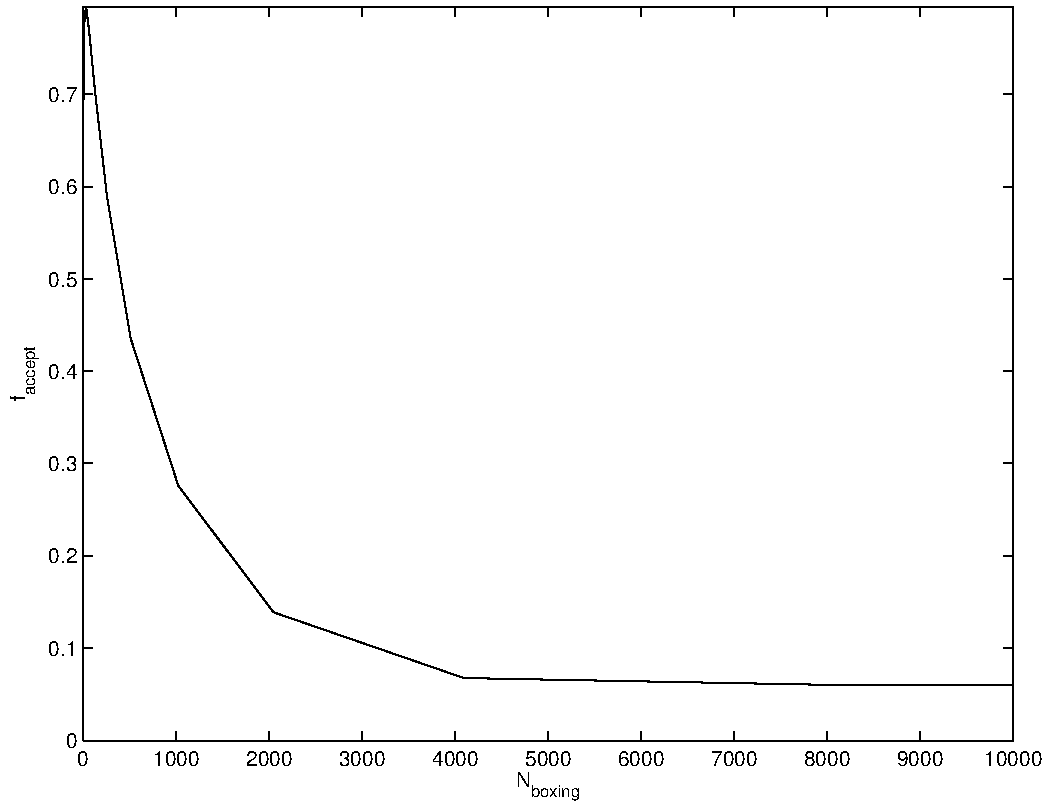
\includegraphics[width=0.8\textwidth]{acceptRate}
  \end{center}
  \caption{\label{fig:acceptRate} The inter-model acceptance rate as a
    function of boxing number for the RJMCMC described in the text.}
\end{figure}

\section{Examples and other uses} \label{sec:examples}

RJMCMC with efficient PDF interpolation via kD trees can be used in a large variety of problems in physics and astronomy, whenever Bayesian analysis is used to perform model selection.  Below, we describe several scenarios in which we have successfully applied this technique.  Moreover, PDF interpolation with a kD tree can be extremely useful in other contexts, beyond a reversible-jump MCMC.  We suggest two examples below: generating efficient jump proposal distributions in a single-model MCMC and convergence tests.


We have successfully employed the RJMCMC technique described above
when evaluating several alternative models for the distribution of the
masses of black holes in X-ray binaries \cite{Farr:2010}.  We
performed a Bayesian analysis of the mass distribution of stellar-mass
black holes using the observed masses of 15 low-mass X-ray binary
systems undergoing Roche lobe overflow and five high-mass, wind-fed
X-ray binary systems.  We considered ten different mass distribution
models: Gaussian, double Gaussian, power law, exponential decay, log
normal, and 1-, 2-, 3-, 4-, and 5-bin histograms.  Each model was
described by between two and six parameters.  Model selection using
RJMCMC with kD trees allowed us to determine that the mass
distribution of the low-mass systems is best fit by a power-law, while
the distribution of the combined sample is best fit by the exponential
model.  Based on the model selection, we were able to determine which
models would provide the best information about astrophysically
relevant parameters, such as the minimum black hole mass.  We were
also able to conclude that the low-mass subsample is not consistent
with being drawn from the distribution of the combined population
\cite{Farr:2010}.

Gravitational-wave astronomy provides the setting for another ongoing
study.  Interesting triggers from the LIGO and Virgo
gravitational-wave detector pipeline that searches for compact binary
coalescences are followed up with Bayesian parameter estimation tools.
In general, several possible models for the data are considered,
including a pure noise model, noise superimposed on a non-spinning
gravitational-wave signal, or noise superimposed on a gravitational
wave signal that includes significant spin or spins in the binary
components.  The models can include a large number of parameters (up
to 15 for the model with two spinning components), and RJMCMC with
interpolation via kD trees is again successful at computing the model
evidences. \ilya{Add references throughout this paragraph.}

As discussed in Section \ref{sec:mcmc}, finding an efficient jump proposal distribution can be a challenge even for a single-model MCMC.  This is particularly difficult when the parameter space is multi-modal, in which case the Markov chain can get stuck on individual high-likelihood islands in the parameter space.  Traversals of low-likelihood oceans by a series of short jumps are extremely unlikely, and random long jumps are almost always rejected, making sampling very inefficient.  Ideally, an analytical understanding of the model that would give a glimpse of the structure of the archipelago of islands would allow for the creation of jump proposal distributions that combine short jumps designed to explore individual islands with directed long jumps that are likely to end up on neighboring islands.  However, it is not always possible to gain such understanding short of performing the MCMC itself.  One solution lies in running multiple chains that explore the parameter space, perhaps getting stuck on local maxima, and then combining the points and interpolating with a kD tree to create a jump proposal distribution.  Although the chains in the first iteration will not have converged, and the relative sizes of the modes will not be accurately known, this will ensure that all of the modes (islands) are at least included in the jump proposal distribution for a second stage, greatly improving its efficiency.  Other modifications to this technique, which we are currently investigating, include multiple iterative stages, with the interpolated samples from each previous stage used as a jump proposal distribution for the next stage, until the posterior PDF is read off from the final stage; and the use of higher temperatures in the early-stage chains to improve sampling.

The possibility of MCMC chains becoming even temporarily stuck on
local maxima also affects convergence.  In the absence of a sufficient
number of jump proposals between the local maxima, the MCMC may not
accurately represent their relative sizes.  For example, this can
happen with antipodal sky location degeneracies for networks of three
ground-based gravitational-wave interferometers or for low-frequency
gravitational wave signals in the proposed space-borne instrument LISA
\cite{LISA}.  Although PDFs produced by MCMC chains will generally
show both locations on the sky, the chain length may not be
sufficiently long in practice to include enough jumps between the two
high-likelihood antipodal locations.  In general, the relative weight
of two separated peaks is determined with a fractional error that
scales as $1/\sqrt{N_{\textnormal{transitions}}}$, where
$N_{\textnormal{transitions}}$ is the number of transitions between
the peaks.  By increasing the number of proposed transitions, the
convergence of such PDFs can be enhanced using the kD tree
interpolated proposal.  We can test the convergence of an MCMC with
local jumps by running a followup MCMC with a jump proposal
distribution from an interpolation of the first MCMC's PDF.  This
follow-up MCMC would make large global jump proposals rather than
small local ones, meaning that it could rapidly accumulate sufficient
points to determine whether the original run spent correct fractional
amounts of time in the various modes.

\section{Conclusion/Discussion}





\nocite{Littenberg2009}

\bibliography{paper}

\end{document}